\documentclass[11pt, oneside]{article} 	% use "amsart" instead of "article" for AMSLaTeX format
\usepackage{geometry} 		% See geometry.pdf to learn the layout options. There are lots.
\geometry{letterpaper}  		% ... or a4paper or a5paper or ... 
\usepackage[parfill]{parskip} 		% Activate to begin paragraphs with an empty line rather than an indent
\usepackage{graphicx}				% Use pdf, png, jpg, or eps§ with pdflatex; use eps in DVI mode
								% TeX will automatically convert eps --> pdf in pdflatex		
\usepackage{amssymb}
\usepackage{amsmath}
\usepackage{authblk}
\usepackage[
backend=biber,
style=alphabetic,
]{biblatex}
\usepackage{graphicx}
\graphicspath{ {./images/} }
\usepackage{verbatim}
\usepackage{tikz} 
\usepackage{subcaption}
\captionsetup{compatibility=false}



\usepackage{syntonly}

% \syntaxonly \langle -- use this for checking syntax only
% \mbox {text} - keep together
% \fbox {text} - keep together and draw around

%\pagestyle{plain|headings|empty} % header and footer p.27
%SetFonts
%\include{filename}, \includeonly{filename1, filename2} , \input[fiename}

%SetFonts% 


\title{Polynomial Uniqueness via Tournaments}
\author{Dave Fetterman}
\affil{Obviously Unemployed}
\date{2/10/23}
\begin{document}
\maketitle

\begin{abstract}

In 2D space, two points $(x_1, y_1), (x_2, y_2), x_1 \neq x_2$ define a line, a polynomial of degree 1.  Three distinct points $(x_1, y_1), (x_2, y_2), (x_3, y_3), x_1 \neq x_2 \neq x_3$ define a parabola, a polynomial of degree 2.  In general, for finite univariate polynomials of nonnegative, whole degree, $n+1$ such points uniquely specify a polynomial of degree $n$.  Why?
\\

This is the farthest thing from a new result. This is a paper is instead a thoroughly awkward trip through a few mathematical domains to arrive at this well known destination. Helicopters and cars both have their uses. But you wouldn't build a car by turning a helicopter on its side and adding wheels.  Metaphorically, I do, so you don't have to.

\end{abstract}

\section{Setup}

If we have points $f(x_0) = y_0, f(x_1) = y_1,  \ldots f(x_{n}) = y_{n}$, how can we determine the coefficients $a_i$ of the polynomial $f(x) = a_0x^0 + a_1x^1 + \ldots + a_nx^n$?

This square matrix of width $n+1$, which I'll denote $X_n$, is known as a Vandermonde matrix\cite{1}, and models this set of $n+1$ equations as $X \cdot \vec{a} = \vec{y}$:

 $\begin{bmatrix}
1 & x_0 & x_0^2 & \ldots & x_0^{n} \\
1 & x_1 & x_1^2 & \ldots & x_1^{n} \\
\vdots & & & & \vdots  \\
1 & x_{n} & x_{n}^2 & \ldots & x_{n}^{n} \\
\end{bmatrix}
\cdot 
\begin{bmatrix}
a_0 \\
a_1 \\
\vdots \\
a_n \\
\end{bmatrix}
=
\begin{bmatrix}
y_0 \\
y_1 \\
\vdots \\
y_{n} \\
\end{bmatrix}
$
\\

Therefore, we can find our unique coefficient vector $A$ if and only if we can solve $X \cdot \vec{a} = \vec{y}$, or $\vec{a} = X^{-1} \vec{y}$.  This has a unique solution if and only if $\det(X) \neq 0$.  The rest of this paper tries to find this determinant through all the wrong ways.

\section{Finding the Vandermonde determinant}

It should be noted that there are other, clearer methods of finding this determinant\cite{1} either starting with polynomial unqiueness (basically, going the ``other'' direction), abstract algebra, direct linear algebra, vector maps, and likely others.  These, however, were not the ones I stumbled on.

First, we know that if any $x_i = x_j$ for distinct $i, j$, we have a zero determinant and no solution. If $f(x_i) = f(x_j), x_i = x_j$, then we are simply underdetermined (not enough points for a unique polynomial).   If $f(x_i) = f(x_j), x_i \neq x_j$, then we have an impossible vertical section of our graph.  Otherwise, we are in good shape.  
\\

This suggests that every pair $(x_i, x_j), i < j$ corresponds to a factor  $(x_j - x_i)$ in the determinant, and that the determinant is then some multiple of $D = \prod_{0 \leq i < j \leq n}(x_j-x_i)$.

Taking $n=2$ as a base case ($n=1$ produces a boring constant $f(x)$), we see that 
 $\det\begin{bmatrix}
1 & x_0  \\
1 & x_1  \\
\end{bmatrix} = (x_1 - x_0)$, suggesting $D$ is the determinant of a Vandermonde matrix.  

\subsection{Setup: Vandermonde inductive step and main theorem}

\fbox{\textbf{Theorem}: The determinant of $X_n$ with generating coefficients $x_0, x_1 ... x_n$ is $\prod_{0 \leq i < j \leq n}(x_j-x_i)$.}

With the base case $n=2$ in hand, the rest of the paper handles the inductive step of proving the main theorem.

\textbf{Inductive Step of Proof of Theorem}:
\\

\fbox{If, for all $X_n$, $\det(X_n) = \prod_{0 \leq i < j \leq n}(x_j-x_i)$, then for all $X_{n+1}, \det(X_{n+1}) = \prod_{0 \leq i < j \leq n + 1}(x_j-x_i)$}.

\subsubsection{Definitions} 

Let's create a few definitions: 
\begin{itemize}
\item Denote by $M_{n,k}$ the Vandermonde matrix  $X_n$ with column $n$ and row $k$ excluded, often called a ``matrix minor''.   \emph{Note: I use zero-indexed matrices in this paper, since in the case of a Vandermonde matrix $X_n$, the zero-indexed entry $(i, j)$ neatly corresponds to $x_i^j$}.
\item Given an ordered set of indices $I = [0, n]$, denote by $P_I$ the product of all factors the form $(x_j - x_i)$, given $i < j$ and $i, j \in I$.  So $P_{[0,2]} = (x_1 - x_0)(x_2-x_0)(x_2- x_1)$.
\item Given an ordered set of indices $I = [0, n]$, denote by $S_I$ the sum over all permutations $\sigma$ of $I$ of $sgn(\sigma) x_{\sigma(n)}^{n} x_{\sigma(n-1)}^{n-1} ... x_{\sigma(0)}^{0} $. So $S_{[0,2]} = x_2^2x_1^1x_0^0 - x_2^2x_0^1x_1^0 - x_1^2x_2^1x_0^0 + x_1^2x_0^1x_2^0 + x_0^2x_2^1x_1^0 - x_0^2x_1^1x_2^0$.
\end{itemize}

\subsubsection{Proof Plan for Inductive Step} 

The rest of the proof of the inductive step above follows from showing:

\begin{itemize}
\item \textbf{P-S Equivalence Lemma}: For a set of indices $I$, $P_I = S_I$.  This is the main statement to prove.
\item (1) $det(X_n) = \sum_{k=0}^n (-1)^{k+n} x_k^n\det(M_{n, k})$ 
\item (2) For our base base, $\det(X_2) = P_{[0,1]}$
\item (3) By inductive hypothesis $det(X_n) = \sum_{k=0}^n (-1)^k x_k^n P_{[0,n] - \{k\}}$
\item (4) $\sum_{k=0}^n (-1)^k x_k^n S_{[0,n] -\{k\}} = S_{[0, n]}$
\item (5) By the Lemma, $\sum_{k=0}^n (-1)^k x_k^n P_{[0,n] -\{k\}} = P_{[0, n]}$
\item (6) Therefore, transitively, $det(X_n) = P_{[0, n]}$.
\end{itemize}

\subsubsection{Straightforward Steps in Proof Plan}

(1) is the minor-based definition of the determinant.

The determinant of 
 $X = \begin{bmatrix}
1 & x_0 & x_0^2 & \ldots & x_0^{n} \\
1 & x_1 & x_1^2 & \ldots & x_1^{n} \\
\vdots & & & & \vdots  \\
1 & x_{n} & x_{n}^2 & \ldots & x_{n}^{n} \\
\end{bmatrix}
$ can be calculated down the rightmost column as

$\det(X) = (-1)^n [ x_0^n \det(M_{n,0}) - x_1^n \det(M_{n,1}) +  ... + (-1)^n x^n \det(M_{n,n})]$.
\\

(2) is clear, with 
$\det(\begin{bmatrix} 1 & x_0 \\ 1& x_1 \end{bmatrix})$
$= -1\cdot(1* M_{1, 1} - 1* M_{1,0}) = $
$(x_1 - x_0) = P_{[0,1]}$.

(3) says inductively, we can presuppose that  for any $M_{n, k}$, \emph{which is itself a Vandermonde matrix of smaller size}, $\det(M_{n,k})$ can be expressed as $P_{[0,n] - \{k\}}$

(4) This simply splits out all terms of the form $sgn(\sigma) x_{\sigma(n)}^{n} x_{\sigma(n-1)}^{n-1} ... x_{\sigma(0)}^{0}$ into those that start with $x_k^n$ and no $x_k$ in the tail, summed over all $k$.   On  $\{c,b,a\}$, for example, the terms split out exactly into $c^2(b^1a^0 - b^0a^1) - b^2(c^1a^0-a^1c^0) + a^2(c^1b^0-b^1c^0) = c^2b^1a^0 - c^2a^0b^1 - b^2c^1a^0 + b^2a^1c^0 + a^2c^1b^0 - a^2b^1c^0$.

(5) follows from applying the $P$-$S$ equivalence Lemma to swap instances of $S$ with those of $P$.

(6) Following the equalities all the way back to 1, $\det(X_n)$ is then $P[0,n]$.

\section{Proof of $P_{[0,n]} = S_{[0,n]}$}

\subsection{Example: $P{[0,1]} = S{[0,1]} \Rightarrow P{[0,2]} = S{[0,2]}$}
We've already established that $P_{[0,1]} = S_{[0,1]}$.  To see that $P_{[0,2]} = S_{[0,2]}$, write it out:

\begin{align}
P_{[0,2]}  \\
= (x_2-x_1)(x_2-x_0)P_{[0,1]} \\
= (x_2-x_1)(x_2-x_0)S_{[0,1]} \\
= x_2^2(x_1^1x_0^0 - x_0^1x_1^0) \\
+ x_2x_0(x_1^1x_0^0 - x_0^1x_1^0) \\
- x_2x_1 (x_1^1x_0^0 - x_0^1x_1^0) \\
+ x_1x_2(x_1^1x_0^0 - x_0^1x_1^0)  \\
= x_2^2x_1^1x_0^0  + x_1^2x_0^1x_2^0 + x_0^2x_2^1x_1^0   \\
 - x_2^2x_0^1x_1^0 - x_1^2x_2^1x_0^0 - x_0^2x_1^1x_2^0 \\
+ x_0^1x_1^1x_2^1 - x_0^1x_1^1x_2^1 \\
= S_{[0,2]}
\end{align}

Note that line (3) follows from line (2) by base case, line (8) is the set of even permutations of $\{2,1,0\}$, line (9) the odds, and line (10) becomes zero.

\subsection{Graph Intuition}

Rather than handle these $2^{\begin{pmatrix}n\\2\end{pmatrix}}$ terms by hand each time algebraically, we'll treat these factors $(x_j - x_i)$ as a \emph{graph}.

The $2^{\begin{pmatrix}n\\2\end{pmatrix}} = 2^{\begin{pmatrix}3\\2\end{pmatrix}} = 8$ terms expanded on lines (8) - (10) are actually the 8 terms resulting from multiplication of the three factors $(x_2 - x_1)(x_2-x_0)(x_1-x_0)$.  This can be mapped to every possible instance of a complete directed graph (also known as a ``tournament'') on 3 nodes, with the edge ``pointing'' from the selected term towards the omitted term in $(x_j - x_i)$.

For example, the term $x_2^2x_1^1x_0$, produced by multiplying the left term of the three factors of $(x_2-x_1)(x_2-x_0)(x_1-x_0)$, corresponds to graph 1a.  Note we use capital $X_1$ to mean that term was selected in $(X_1 - x_2)$ for example.


\begin{figure}
\centering
\begin{subfigure}{.5\textwidth}
  \centering
  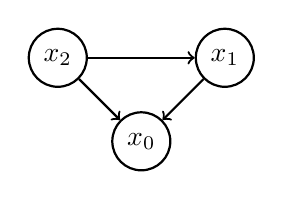
\begin{tikzpicture}[node distance={15mm}, thick, main/.style = {draw, circle}] 
\node[main] (1) {$x_0$}; 
\node[main] (2) [above right of=1] {$x_1$}; 
\node[main] (3) [above left of=1] {$x_2$}; 
\draw[->] (3) -- (2); 
\draw[->] (3) -- (1);
\draw[->] (2) -- (1);
\end{tikzpicture}
  \caption{($X_2-x_1)(X_2-x_0)(X_1-x_0) = x_2^2x_1^1x_0^0$}
  \label{fig:sub1}
\end{subfigure}

\begin{subfigure}{.5\textwidth}
  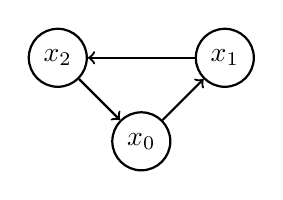
\begin{tikzpicture}[node distance={15mm}, thick, main/.style = {draw, circle}] 
\node[main] (1) {$x_0$}; 
\node[main] (2) [above right of=1] {$x_1$}; 
\node[main] (3) [above left of=1] {$x_2$}; 
\draw[<-] (3) -- (2); 
\draw[->] (3) -- (1);
\draw[<-] (2) -- (1);
\end{tikzpicture}

  \caption{($x_2-X_1)(X_2-x_0)(x_1-X_0)= x_2^1x_1^1x_0^1$}
  \label{fig:sub2}
\end{subfigure}

\begin{subfigure}{.5\textwidth}
  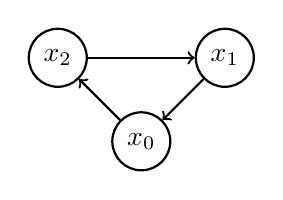
\begin{tikzpicture}[node distance={15mm}, thick, main/.style = {draw, circle}] 
\node[main] (1) {$x_0$}; 
\node[main] (2) [above right of=1] {$x_1$}; 
\node[main] (3) [above left of=1] {$x_2$}; 
\draw[->] (3) -- (2); 
\draw[<-] (3) -- (1);
\draw[->] (2) -- (1);
\end{tikzpicture}

  \caption{($X_2-x_1)(x_2-X_0)(X_1-x_0) = -x_2^1x_1^1x_0^1$}
  \label{fig:sub3}
\end{subfigure}


\caption{Three terms of  $P_{[0,2]}$, corresponding to complete directed graphs of size 3}
\label{fig:test}
\end{figure}

The term $x_2^1x_1^1x_0^1$, from multiplying the right, left, and right terms of the above product respectively, corresponds to 1b.  And the inverted sequence left, right, left, produces the inverted cycle and algebraic inverse $-x_2^1x_1^1x_0^1$ in 1c.

This should give a flavor of the proof.
\subsection{P-S Equivalence Lemma Proof layout}

Here is a layout of the proof that $P_I=S_I$.

First, we prove a set of lemmas:
\begin{itemize}
\item (1) Lemma: The set of terms in an expanded $P_{[0,n]} =\prod_{0 \leq i < j \leq n}(x_j - x_i)$ can be mapped 1:1 to the set of all possible directed complete graphs.
\item (2) Lemma :All directed complete graphs are either acyclic or contain a 3-cycle.
\item (3) Lemma: Acyclic graphs correspond through the above bijection with terms of the form $sgn(\sigma) x_{\sigma(n)}^nx_{\sigma(n-1)}^{n-1}  ... x_{\sigma(0)}^{0}$ for some permutation $\sigma$ on $[0,n]$.
\item (4) Lemma: Cyclic tournaments with a 3-cycle can be uniquely paired 1:1 with an otherwise identical graph with that 3-cycle inverted.
\end{itemize}

Through these lemmas, we can start with a base case equality $P_{[0,2]} = S_{[0,2]}$ and show:
\begin{itemize}
\item (5) This bijection maps all possibilities of adding an additional node $x_n$ to an acyclic graph $G$ of $n-1$ nodes to multiplying $\prod_{0 \leq i < n}(x_n-x_i)$ by $P_{[0,n-1]}$
\item (6) This bijection maps all possibilities of adding an additional node $x_n$ to an acyclic graph $G$ of $n-1$ nodes to $S_{[0,n]}$.
\item (7) Therefore, $P_{[0,n]} = S_{[0,n]}$
\end{itemize}

\subsection{Lemma 1}

Every possible complete directed graph  $G = (E,V)$ of vertex size $n$  consists exactly of edges $(i \rightarrow j)$ with $i, j \in [v_0, v_n-1], i < j$.  If $(i \rightarrow j) \in E$, then consider $(X_i - x_j)$ in the expansion of $P_{[0, n-1]}$; otherwise if $(j \rightarrow i) \in E$, then consider $(x_i - X_j)$ in the expansion of $P_{[0, n-1]}$.  Conversely, if $(X_i - x_j)$ is in a term of $P_{[0, n-1]}$, take $(i \rightarrow j)$ for an edge in the graph, otherwise $(j \rightarrow i)$.  As in Figure 1, this isomorphism should be clear.

\subsection{Lemma 2}

If the graph contains no cycles, or a cycle of length 3, we are done.

If a graph contains some cycle $(v_0 \rightarrow v_{1} \rightarrow  ...  \rightarrow v_{m-1} \rightarrow  v_0)$ of length $m > 3$, we can split it into two possible cycles: $A = (v_0 \rightarrow  v_{1} \rightarrow v_{2} \rightarrow  v_0)$ and $B = (v_{2} \rightarrow  v_{3} \rightarrow  ... \rightarrow v_{0} \rightarrow v_{2} )$.  Depending on the direction of edge $(v_{0}, v_{2})$, exactly one of $A$ or $B$ must be a cycle of smaller length.  If $A$ is a cycle, we are done.  Else use $B$ and reapply recursively, eventually down to a cycle of length 3.

\subsection{Lemma 3}

Another way of saying ``every acyclic tournament maps through some $\sigma$ to$sgn(\sigma) x_{\sigma(n)}^nx_{\sigma(n-1)}^{n-1}  ... x_{\sigma(0)}^{0}$ is ``No acyclic tournament has nodes of equal degree''.  For example, an acyclic tournament on a set of nodes indexed $[0, 3]$ necessarily looks like the following:

  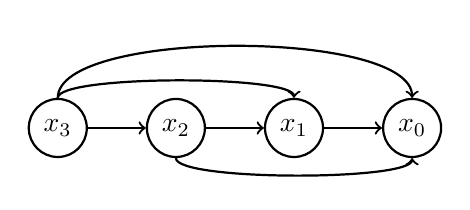
\begin{tikzpicture}[node distance={15mm}, thick, main/.style = {draw, circle}] 
\node[main] (4) {$x_3$}; 
\node[main] (3) [right of=4] {$x_2$}; 
\node[main] (2) [right of=3] {$x_1$}; 
\node[main] (1) [right of=2] {$x_0$}; 
\draw[->] (4) -- (3); 
\draw[->] (4) to [out = 90, in = 90, looseness=.25] (2);
\draw[->] (4) to [out = 90, in = 90, looseness=.5] (1);
\draw[->] (3) to [out = 270, in = 270, looseness=.25] (1);
\draw[->] (3) -- (2);
\draw[->] (2) -- (1);
\end{tikzpicture}

Every node has a unique out degree, ranging from $n-1$ to 0.  (Note: This graph corresponds to the term $x_3^3x_2^2x_1^1x_0^0$).  As every edge ``goes right'', it's clear that there can be no cycle (or particularly, 3-cycle) here.

For the converse, consider the statement that ``no acyclic tournament has a subgraph (removing vertices) with two or more vertices of equal degree''.  If this is true then certainly the graph has to have the above form out outdegrees.  To see this:

\begin{itemize}
\item If the graph is of the form $sgn(\sigma) x_{\sigma(n)}^nx_{\sigma(n-1)}^{n-1}  ... x_{\sigma(0)}^{0}$ for some $n$ and some $\sigma$, we are done.
\item Suppose then it has two vertices with duplicate outdegrees, but has no cycles. Eliminate vertices, starting from $x_n$, then $x_{n-1}$, down to $x_2$ just until a subgraph is of the form with all unique outdegrees, which we'll call $y_{m} ... y_0$, with $y_m$ of outdegree $m$ and $y_0$ of outdegree 0.  Call $y_0$ for now $y^-$.
\item Add the last removed vertex $y^*$ and its edges back.  $y^*$ must have the same outdegree as some other vertex, otherwise we have a contradiction.
\item Step: If $(y^- \rightarrow y^*)$ is in the graph, then necessarily there is a cycle $(y^- \rightarrow y^* \rightarrow $ some $y_j \rightarrow y^-)$, so we have a contradiction.
\item Else $(y^* \rightarrow y^-)$ is in the graph, so the outdegree of $y^*$ can't be 0.  Remove $y^-$, reducing all vertices by outdegree 1, creating a new $y^- \neq y^*$ with minimum degree, and go back to (Step).
\end{itemize}

From this, we can conclude that an acylic directed tournament has vertices of all unique degrees, and thus, up to vertex labeling (permutation), has the form $sgn(\sigma) x_{\sigma(n)}^nx_{\sigma(n-1)}^{n-1}  ... x_{\sigma(0)}^{0}$  for some $\sigma$.

\subsection{Lemma 4}

Suppose, for a graph $G$ we fix an ordering of vertices like $\{x_n, x_{n-1}, x_{n-2}... x_0\}$.  Suppose $(x_a, x_b, x_c)$ is the 3-cycle with highest lexicographic order ($x_n > x_{n-1} > ...$), with edges pointing either direction.  Then, the graph $G'$, with the same edges, except the direction of cycle  $(x_a, x_b, x_c)$ reversed:
\begin{itemize}
\item (1) Is a dual to $G$.
\item (2) Has a representation through the main bijection which is an inverse to that of G.
\end{itemize}

(1) is clear because each uniquely determines the other; the order of vertices is the same, thus the ``first'' cycle is the same, and the order need only be reversed.
\\
(2) Inverting $(X_1 - x_2)(X_2-x_3)(X_3-x_1) = X_1X_2X_3$ yields $(x_1 - X_2)(x_2-X_3)(x_3-X_1) = -X_1X_2X_3$, for any choice of $x_1, x_2, x_3$




\section{Pieceyard}


 
Base Case: We've shown this is true for  $n=2 \Rightarrow S_{[0,1]} = (x_1^1x_0^0 - x_0^1x_1^0)$.  
So our inductive step supposes that all terms of (3) for ranges $[0, n-1]$ are of the form  $sgn(\sigma) x_{\sigma(n-1)}^{n-1} x_{\sigma(n-2)}^{n-2} ... x_{\sigma(0)}^{0} $ for some permutation $\sigma$ on the node set $[0, n-1]$.  

The proof that  $S_[0,n] = \prod_{0 \leq i < j \leq n} (x_j - x_i)$ requires adding a new node $x_n$ to the left side and a multiplying new set of factors $\prod_{0 \leq i < \leq n} (x_n - x_i)$ by the right side and showing they are equal.

So, for example, we know that $P_{[0,1]} = (x_1 - x_0) = x_1^1x_0^0 - x_0^1x_1^0 = S_{[0,1]}$.
We can use this to show $P_{[0,2]} = (x_2 - x_1)(x_2-x_0)P_{[0,1]} = x_2^2-x_2x_1-x_2x_0$

\begin{itemize}
\item Lemma 1: Show an isomorphism between products of the form (3) and tournament graphs on $n+1$ nodes.
\item Lemma 2: Show that terms of the form $sgn(\sigma) x_{\sigma(n)}^n x_{\sigma(n-1)}^{n-1} ... x_{\sigma(0)}^{0} $ remain in (3) after expansion.  These correspond to acyclic tournaments on $n+1$ nodes.
\item Lemma 3: Show that all other terms in the expansion of (3), which correspond to tournaments with a cycle, can be paired 1:1 with a identical but inverted term, corresponding to an identical graph with \emph{one 3-cycle reversed}.
\item Thus, the sum of the terms addressed 
\end{itemize}

\section{Prove : VanDerMonde matrix determinant is prod $(x_i - x_j), 1 <= i < j <= n$}
 This is the determinant of the van der modne matrix
\subsection{Base cane: n = 2}
\subsection{Inductive case} This equals$ x^n$ (product without x), +$ y^n $(product without y)...
\begin{comment}
- Represent as a graph tournament, n nodes, (n choose 2) edges.  There are 2^(n choose 2) possibilities.
- Each term (+/-) x_0^a_0*x_1^a_1...*x_n^a_n, where sum a_i = (n choose 2), represents one possible tournament on a directed complete graph of size n
- If there are no cycles in a given tournamnet
  - then it's of the form b^n c^n-1 ... x^1 y^0 for some b,c,...y in x_i.
- If there are ctycles in a tournament
  - Any even cycle implies an odd cycle (quick proof)
  - Therfore there's an odd cycle
  - Reversing an odd cycle produces a different graph with an odd cycle and flipped sign.
- For a tournament config that is NOT a topo sort (has a cycle)
  - There are as many positivies as negatives (PROVE?)
  - So the terms cancel out
  - Therefore everything is of the form b^n c^n-1 ... x^1 y^0
  - So big product up to n is x^n(prodcut without x) + y^n(product without y..).
*** This is zero if and only if x_i = x_j for some
*** Therefore, only one solution for n distinct points on a polynomial of size n.

\end{comment}


By inductive hypothesis, each of the terms $x_k^n\det(M_{n,k})$ becomes:

$x_k^n\prod_{0 \leq i < j \leq n; i \neq k, j \neq k} (x_j - x_i)$ 
or 
$x_k^n\prod_{0 \leq i < j \leq n; i, j \in I_{n-{k}}} (x_j - x_i)$ 


Therefore, we need to prove that $0 \neq \det(X)$

\begin{align}
= \sum_{k=0}^n (-1)^k x_k^n\det(M_{n, k}) \\
= \sum_{k=0}^n (-1)^k x_k^n\Big[\prod_{0 \leq i < j \leq n; i, j \in [0,n] - \{k\}} (x_j - x_i) \Big] \\
=\prod_{0 \leq i < j \leq n; i, j \in [0,n]} (x_j - x_i) 
\end{align}

(1) is a determinant expansion.  The $det$ term equals the bracketed term of (2) by inductive hypothesis.



We seek to prove this main theorem:

\textbf{Theorem}: The expansion of (3) is exactly the sum of all possible terms of the form $sgn(\sigma) x_{\sigma(n-1)}^{n-1} x_{\sigma(n-2)}^{n-2} ... x_{\sigma(0)}^{0} $ for some permutation $\sigma$ on the node set $[0, n-1]$.  Call this $S_{[0,n]}$.  So, for example$S_{\{d,c,b,a\}}$, would be exactly all terms like $d^3c^2b^1a^0$, $-c^3d^2b^1a^0$ or $-c^3a^2d^1b^0$.

\emph{If we have this theorem proven}, then:

\begin{itemize}
\item For $n=2$, the determinant of $X_2$ is $1\cdot x_1 - 1 \cdot x_0 = (x_1^1x_0^0 - x_0^1x_1^0) = S_{[0,1]}$
\item By inductive hypothesis, the expansion of the bracketed term of (2), $S_{[0,n]-\{k\}}$ yields the same set of sums except each sum excludes all use of $x_k$.
\item The sum of all terms $(-1)^kx_k^nS_{[0,n]-{k}}$ is exactly $S_{[0,n]}$, meaning (3).
\item Therefore, (2) = (3) and we have our Vandermonde determinant (and thus  our proof of polynomial uniquenss).
\end{itemize}


% Graph drawing reference: https://www.baeldung.com/cs/latex-drawing-graphs


\begin{figure}
\centering
\begin{subfigure}{.5\textwidth}
  \centering
  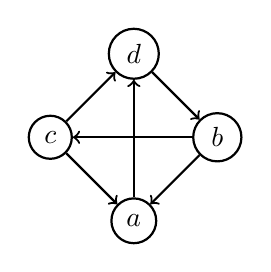
\begin{tikzpicture}[node distance={15mm}, thick, main/.style = {draw, circle}] 
\node[main] (1) {$a$}; 
\node[main] (2) [above right of=1] {$b$}; 
\node[main] (3) [above left of=1] {$c$}; 
\node[main] (4) [above right of=3] {$d$}; 
\draw[<-] (4) -- (3); 
\draw[->] (4) -- (2); 
\draw[<-] (4) -- (1); 
\draw[<-] (3) -- (2); 
\draw[->] (3) -- (1);
\draw[->] (2) -- (1);
\end{tikzpicture}

  \caption{An arbitrary tournament on 4 nodes}
  \label{fig:sub1}
\end{subfigure}
\begin{subfigure}{.5\textwidth}
  \centering
    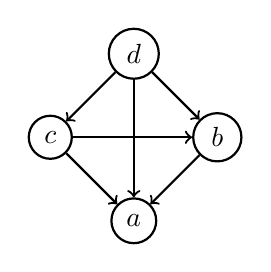
\begin{tikzpicture}[node distance={15mm}, thick, main/.style = {draw, circle}] 
\node[main] (1) {$a$}; 
\node[main] (2) [above right of=1] {$b$}; 
\node[main] (3) [above left of=1] {$c$}; 
\node[main] (4) [above right of=3] {$d$}; 
\draw[->] (4) -- (3); 
\draw[->] (4) -- (2); 
\draw[->] (4) -- (1); 
\draw[->] (3) -- (2); 
\draw[->] (3) -- (1);
\draw[->] (2) -- (1);
\end{tikzpicture}
  \caption{An (acyclic) tournament $d^3c^2b^1a^0$}
  \label{fig:sub2}
\end{subfigure}
\caption{Tournaments}
\label{fig:test}
\end{figure}



The sorted tournament $d^3c^2b^1a^0$

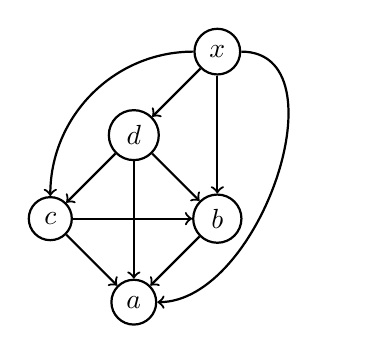
\begin{tikzpicture}[node distance={15mm}, thick, main/.style = {draw, circle}] 
\node[main] (1) {$a$}; 
\node[main] (2) [above right of=1] {$b$}; 
\node[main] (3) [above left of=1] {$c$}; 
\node[main] (4) [above right of=3] {$d$}; 
\node[main] (5) [above right of=4] {$x$}; 
\draw[->] (5) -- (4);
\draw[->] (5) to [out=180, in=90, looseness=1] (3); 
\draw[->] (5) -- (2);
\draw[->] (5) to [out=0, in=0, looseness=1] (1); 
\draw[->] (4) -- (3); 
\draw[->] (4) -- (2); 
\draw[->] (4) -- (1); 
\draw[->] (3) -- (2); 
\draw[->] (3) -- (1);
\draw[->] (2) -- (1);
\end{tikzpicture}

The sorted tournament $x^4d^3c^2b^1a^0$



\begin{figure}
\centering
\begin{subfigure}{.5\textwidth}
  \centering
  
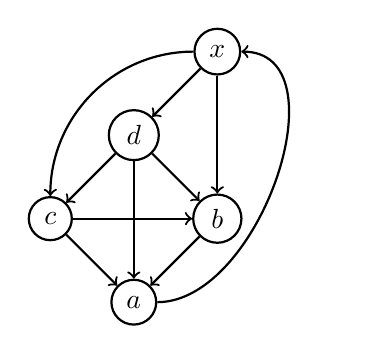
\begin{tikzpicture}[node distance={15mm}, thick, main/.style = {draw, circle}] 
\node[main] (1) {$a$}; 
\node[main] (2) [above right of=1] {$b$}; 
\node[main] (3) [above left of=1] {$c$}; 
\node[main] (4) [above right of=3] {$d$}; 
\node[main] (5) [above right of=4] {$x$}; 
\draw[->] (5) -- (4);
\draw[->] (5) to [out=180, in=90, looseness=1] (3); 
\draw[->] (5) -- (2);
\draw[->] (1) to [out=0, in=0, looseness=1] (5);
\draw[->] (4) -- (3); 
\draw[->] (4) -- (2); 
\draw[->] (4) -- (1); 
\draw[->] (3) -- (2); 
\draw[->] (3) -- (1);
\draw[->] (2) -- (1);
\end{tikzpicture}
  \caption{$-x^3a \cdot d^3c^2b^1a^0$, with cycle $(x b a)$}
  \label{fig:sub1}
\end{subfigure}%
\begin{subfigure}{.5\textwidth}
  \centering
  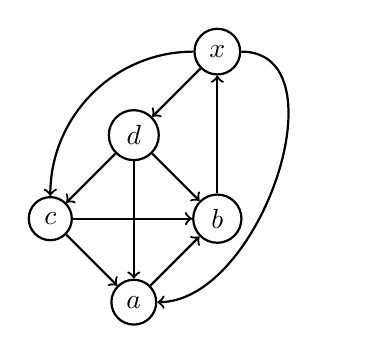
\begin{tikzpicture}[node distance={15mm}, thick, main/.style = {draw, circle}] 
\node[main] (1) {$a$}; 
\node[main] (2) [above right of=1] {$b$}; 
\node[main] (3) [above left of=1] {$c$}; 
\node[main] (4) [above right of=3] {$d$}; 
\node[main] (5) [above right of=4] {$x$}; 
\draw[->] (5) -- (4);
\draw[->] (5) to [out=180, in=90, looseness=1] (3); 
\draw[<-] (5) -- (2);
\draw[->] (5) to [out=0, in=0, looseness=1] (1);
\draw[->] (4) -- (3); 
\draw[->] (4) -- (2); 
\draw[->] (4) -- (1); 
\draw[->] (3) -- (2); 
\draw[->] (3) -- (1);
\draw[<-] (2) -- (1);
\end{tikzpicture}

  \caption{$-x^3b \cdot -d^3c^2a^1b^0$, with cycle $(x a b)$}
  \label{fig:sub2}
\end{subfigure}
\caption{Terms in expanded $\prod (x_j - x_i)$ are inverses with inverted 3-cycles }
\label{fig:test}
\end{figure}







Factors of $(x-a)(x-b)(x-c)(x-d)$ multiplied by $\sigma = d^3c^2b^1a^0$

\begin{center}
\begin{tabular}{||c c c c c||} 
 \hline
 Factor & Product & Matching Factor & Matching $\sigma$ & Critical pair \\ [0.5ex] 
 \hline\hline
 $x^4$ & $x^4d^3c^2b^1a^0$ & none & none & none \\ 
 \hline
 $-x^3a$ & $-x^3d^3c^2b^1a^1$ & $-x^3b$ & $-d^3c^2a^1b^0$ & $ba$ \\ 
 \hline
 $-x^3b$ & $-x^3d^3c^2b^2a^0$ & $-x^3c$ & $-d^3b^2c^1a^0$ & $cb$ \\ 
 \hline
 $-x^3c$ & $-x^3d^3c^3b^1a^0$ & $-x^3d$ & $-c^3d^2b^1a^0$ & $dc$ \\ 
 \hline
 $-x^3d$ & $-x^3d^4c^2b^1a^0$ & none & none & none \\ 
 \hline
 $x^2ba$ & $x^2d^3c^2b^2a^1$ & $x^2ca $& $-d^3b^2c^1a^0$ &  $cb$ \\ 
  \hline
 $x^2ca$ & $x^2d^3c^3b^1a^1$ & $x^2da $& $-c^3d^2b^1a^0$ &  $dc$ \\ 
 \hline
 $x^2da$ & $x^2d^4c^2b^1a^1$ & $x^2db $& $-d^3c^2a^1b^0$ &  $ba$ \\ 

 \hline
 $x^2cb$ & $x^2d^3c^3b^2a^0$ & $x^2db $& $-c^3d^2b^1a^0$ &  $dc$ \\ 
 \hline
 $x^2db$ & $x^2d^4c^2b^2a^0$ & $x^2dc $& $-d^3b^2c^1a^0$ &  $dc$ \\ 
 
 
\hline
 $x^2dc$ & $x^2d^4c^3b^1a^0$ & none & none &  none \\ 
 
 \hline
 $-xcba$ & $-xd^3c^3b^2a^1$ & $-xdba $& $-c^3d^2b^1a^0$ &  $dc$ \\ 

 \hline
 $-xdba$ & $-xd^4c^2b^2a^1$ & $-xcba $& $-d^3b^2c^1a^0$ &  $cb$ \\ 

 \hline
 $-xdca$ & $-xd^4c^3b^1a^1$ & $-xdcb $& $-d^3c^2a^1b^0$ &  $ba$ \\ 

 \hline
 $-xdcb$ & $-xd^4c^3b^2a^0$ & none & none &  none \\ 
 
 
 \hline
 $dcba$ & $ d^4c^3b^2a^1 $ & none & none &  none \\ 
 
 \hline
\end{tabular}
\end{center}


\section{TODO}
\subsection{TODO}

\begin{thebibliography}{9}
\bibitem{1}
Wikipedia: \url{https://en.wikipedia.org/wiki/Vandermonde_matrix}
\end{thebibliography}


\end{document}

